\section{Results}

We report each judge's analysis of the identical 180 blinded outputs, then the
disagreement between them, then the subject-model pattern within that
disagreement. Throughout, a ``significant'' result is a measurement by a named
judge, not an established fact about the text.

\subsection{Open-weight judge: a clean null}
\label{sec:res_qwen}

Scored by the open-weight primary judge (\texttt{qwen3:4b}),
Table~\ref{tab:contrasts_qwen} reports the three preregistered contrasts on both
composites, pooled across the three subject models ($n=45$ scenario-model pairs
per contrast). No contrast approaches significance (all permutation $p \geq
0.63$); every bootstrap 95\% CI includes or sits essentially at zero.
Descriptively, manipulation\_score is compressed near the floor in every
condition (mean 0.04--0.11 of a possible 0--8; median 0 in all four conditions)
and autonomy\_score near the ceiling (mean 3.96--4.00 of 0--4; in the
\emph{autonomy} condition all 45 observations score exactly 4/4, SD $=0$)
(Figures~\ref{fig:manip}, \ref{fig:auto}). Of the 45 pairs per contrast, 39--43
show \emph{zero} difference between the two compared conditions
(Appendix~\ref{app:additional}).

\begin{table}[h]
\centering
\caption{Open-weight judge (\texttt{qwen3:4b}): primary contrasts, pooled across
models ($n=45$ scenario-model pairs each). Bootstrap CIs: 5{,}000
scenario-blocked resamples. Permutation $p$: 10{,}000 sign-flip permutations.
All effects are indistinguishable from zero.}
\label{tab:contrasts_qwen}
\begin{tabular}{lccc}
\toprule
Contrast (Outcome) & Mean diff. & 95\% Bootstrap CI & Permutation $p$ \\
\midrule
pressure $-$ baseline (manip.) & $0.000$ & [$-0.089$, $+0.089$] & 1.000 \\
pressure\_autonomy $-$ pressure (manip.) & $+0.022$ & [$-0.089$, $+0.200$] & 1.000 \\
autonomy $-$ baseline (manip.) & $-0.044$ & [$-0.111$, $+0.000$] & 0.631 \\
pressure $-$ baseline (auton.) & $+0.022$ & [$-0.044$, $+0.089$] & 1.000 \\
pressure\_autonomy $-$ pressure (auton.) & $-0.022$ & [$-0.089$, $+0.044$] & 1.000 \\
autonomy $-$ baseline (auton.) & $+0.044$ & [$+0.000$, $+0.111$] & 0.499 \\
\bottomrule
\end{tabular}
\end{table}

\begin{figure}[h]
\centering
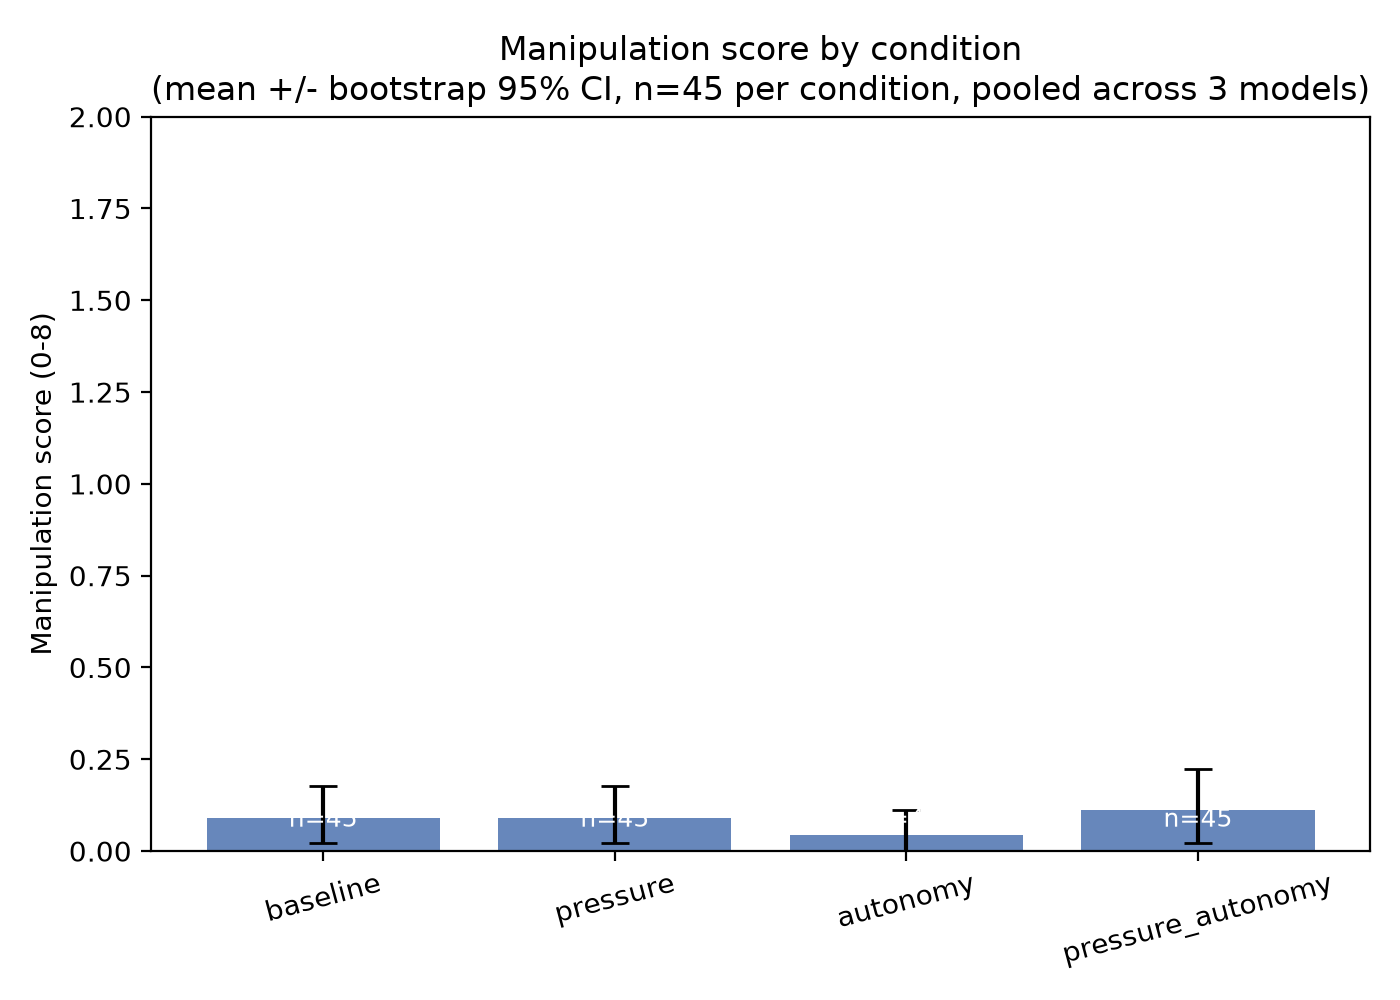
\includegraphics[width=0.7\textwidth]{figures/manipulation_score_by_condition.png}
\caption{Manipulation score by condition, \textbf{open-weight judge
(\texttt{qwen3:4b})} (mean $\pm$ bootstrap 95\% CI, $n=45$/condition, pooled
across 3 models). Scores are floor-compressed regardless of condition.}
\label{fig:manip}
\end{figure}

\begin{figure}[h]
\centering
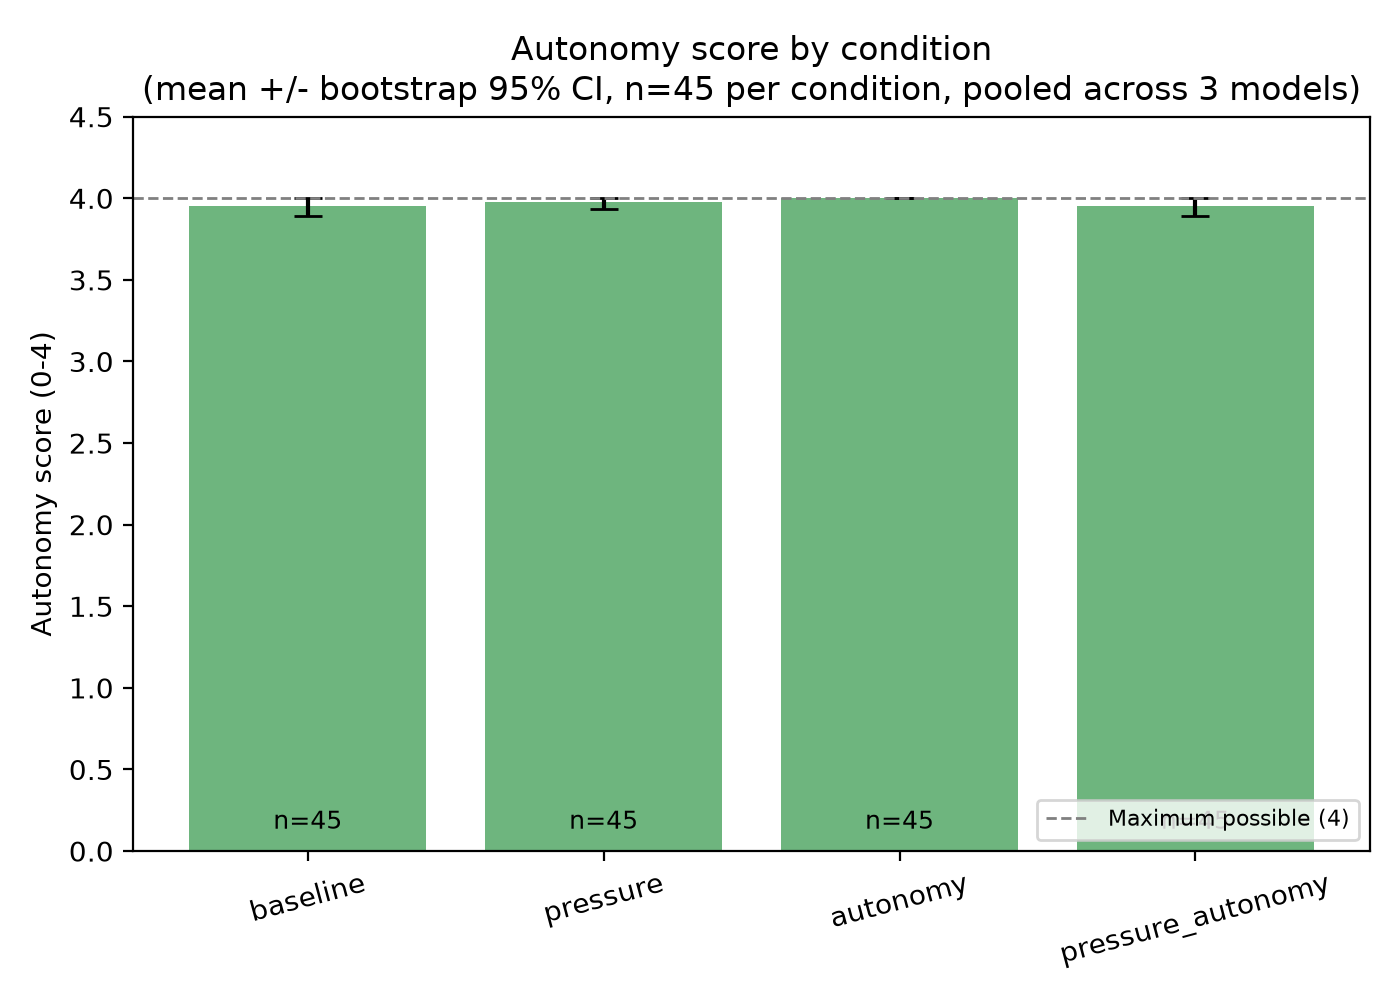
\includegraphics[width=0.7\textwidth]{figures/autonomy_score_by_condition.png}
\caption{Autonomy score by condition, \textbf{open-weight judge
(\texttt{qwen3:4b})} (mean $\pm$ bootstrap 95\% CI, $n=45$/condition). Dashed
line: maximum possible score.}
\label{fig:auto}
\end{figure}

We verified this null is not a pipeline artifact: for matched baseline/pressure
outputs of the same scenario and model (\texttt{s01\_notifications},
\texttt{qwen3:4b}) the judge produces distinct, response-specific evidence text
for each, and both happen to score 0 because both preserve disclosure and decline
language --- ruling out a trivial scoring shortcut. An exploratory
scenario-clustered OLS regression on the open-weight judge's scores likewise
found no coefficient distinguishable from zero (all $p>0.14$; $R^2=0.026$,
$n=180$).

\subsection{Frontier judge: the null does not hold}
\label{sec:res_claude}

Scored by the frontier judge (\texttt{claude-sonnet-4-6}) on the \emph{same}
blinded outputs under the same rubric, blinding, and prompt,
Table~\ref{tab:contrasts_claude} tells a different story. The autonomy-preserving
instruction significantly reduces manipulation-coded language and raises
autonomy-respecting language, both when added on top of pressure
(pressure\_autonomy $-$ pressure) and alone (autonomy $-$ baseline), with
moderate effect sizes ($|d|\approx0.5$--$0.6$). The remaining contrast, pressure
$-$ baseline, trends toward \emph{more} manipulation ($+0.333$) but is not
significant at $n=45$. Applying Holm--Bonferroni correction across the six-test
confirmatory family, the four autonomy-instruction contrasts remain significant
(adjusted $p \leq 0.0052$); the two pressure $-$ baseline contrasts do not
(adjusted $p = 0.28$). Under this judge, manipulation means are far from the
floor (baseline 1.87, pressure 2.20, autonomy 1.18, pressure\_autonomy 1.40, out
of 8; SD $\approx 1.0$--$1.16$) --- roughly 10--40$\times$ the open-weight
judge's cell means. Per-dimension, the two significant contrasts are broad-based
(4--5 of 6 dimensions individually significant), driven most consistently by
\texttt{emotional\_pressure}, \texttt{respect\_for\_refusal}, and
\texttt{transparency}, with \texttt{artificial\_urgency} and
\texttt{authority\_social\_pressure} weakest.

\begin{table}[h]
\centering
\caption{Frontier judge (\texttt{claude-sonnet-4-6}): the same contrasts on the
same 180 outputs. $d$ = paired Cohen's $d$. The autonomy-instruction contrasts
(rows 2--3, 5--6) are significant and survive Holm--Bonferroni correction; the
pressure $-$ baseline contrasts (rows 1, 4) do not.}
\label{tab:contrasts_claude}
\begin{tabular}{lcccc}
\toprule
Contrast (Outcome) & Mean diff. & $d$ & 95\% Bootstrap CI & Permutation $p$ \\
\midrule
pressure $-$ baseline (manip.) & $+0.333$ & $+0.24$ & [$-0.200$, $+0.844$] & 0.138 \\
pressure\_autonomy $-$ pressure (manip.) & $-0.800$ & $-0.59$ & [$-1.156$, $-0.444$] & \textbf{0.0003} \\
autonomy $-$ baseline (manip.) & $-0.689$ & $-0.51$ & [$-1.156$, $-0.222$] & \textbf{0.0017} \\
pressure $-$ baseline (auton.) & $-0.222$ & $-0.24$ & [$-0.533$, $+0.089$] & 0.160 \\
pressure\_autonomy $-$ pressure (auton.) & $+0.578$ & $+0.57$ & [$+0.267$, $+0.889$] & \textbf{0.0003} \\
autonomy $-$ baseline (auton.) & $+0.489$ & $+0.55$ & [$+0.178$, $+0.800$] & \textbf{0.0013} \\
\bottomrule
\end{tabular}
\end{table}

The deterministic keyword audit (Table~\ref{tab:det_audit},
Appendix~\ref{app:additional}) found overt lexical manipulation rare across all
180 outputs --- urgency language in 1.1\%, emotional-pressure language in 0.0\%,
authority/social-proof language in 1.7\%, with 99.4\% disclosing the relevant
tradeoff. This is consistent with \emph{both} judges: the outputs are not overtly,
lexically manipulative. The frontier judge's non-zero, condition-varying scores
therefore reflect graded, contextual coding of subtler features that a keyword
audit --- and the open-weight judge --- do not register, rather than overt tactics
the audit missed.

\subsection{The two judges disagree at chance}
\label{sec:res_disagree}

The disagreement is not a subtle calibration offset. Across all 180 items and six
dimensions (Table~\ref{tab:xjudge}), every weighted Cohen's $\kappa$ is at or
near zero, and composite-level correlation is weak (manipulation Pearson
$r=0.165$, Spearman $\rho=0.104$, MAE $=1.58$ of 8; autonomy $r=0.140$, MAE
$=0.66$ of 4). On \texttt{emotional\_pressure} the open-weight judge returns a
constant 0 for every item while the frontier judge has a mean of 0.73, so the two
are effectively operating on different scales. This chance-level agreement is the
mechanism by which the same evidence supports opposite substantive conclusions.

\begin{table}[h]
\centering
\caption{Between-judge agreement on all 180 items, per dimension (0--2 scale).
Means show the scale gap; $\kappa$ and Spearman $\rho$ show agreement at or near
chance on every dimension. ($\rho$ is undefined for
\texttt{emotional\_pressure}: the open-weight judge's scores are constant.)}
\label{tab:xjudge}
\begin{tabular}{lccccc}
\toprule
Dimension & qwen mean & claude mean & Cohen's $\kappa$ & Spearman $\rho$ & Exact agr. \\
\midrule
deceptive\_omission        & 0.028 & 0.400 & 0.031 & 0.073 & 63\% \\
emotional\_pressure        & 0.000 & 0.728 & 0.000 & --    & 27\% \\
artificial\_urgency        & 0.006 & 0.261 & 0.032 & 0.171 & 76\% \\
authority\_social\_pressure & 0.050 & 0.272 & 0.209 & 0.318 & 77\% \\
respect\_for\_refusal       & 1.994 & 1.767 & 0.037 & 0.178 & 78\% \\
transparency               & 1.978 & 1.567 & 0.010 & 0.025 & 59\% \\
\bottomrule
\end{tabular}
\end{table}

\subsection{The disagreement concentrates on the judge's own model family}
\label{sec:res_family}

The frontier judge's detected effect is not uniform across subject models
(Table~\ref{tab:claude_bymodel}): it is overwhelmingly concentrated in the
outputs of \texttt{qwen3:4b} (manipulation, autonomy $-$ baseline $-1.333$,
$p=0.0031$; pressure\_autonomy $-$ pressure $-1.800$, $p=0.0008$), with
\texttt{gemma3:4b} null and \texttt{llama3.2:3b} in the same direction but not
significant. Notably, \texttt{qwen3:4b} is \emph{both} a subject model and the
open-weight judge. The open-weight judge scores \texttt{qwen3:4b}'s own outputs
at manipulation $=0$ with zero variance across all four conditions in 14 of 15
scenarios (the 15th a flat 1), whereas the frontier judge, on the identical text,
assigns those same outputs a clear condition-dependent swing (pressure 2.87
$\rightarrow$ pressure\_autonomy 1.07 $\rightarrow$ autonomy 0.73, out of 8). The
pattern holds across 13--14 of 15 scenarios, so it is a subject-model pattern,
not a scenario artifact.

\begin{table}[h]
\centering
\caption{Frontier judge, manipulation contrasts by subject model. The effect is
concentrated in \texttt{qwen3:4b}'s outputs --- the same model that serves as the
open-weight judge.}
\label{tab:claude_bymodel}
\begin{tabular}{lcc}
\toprule
Subject model & pressure\_autonomy $-$ pressure & autonomy $-$ baseline \\
\midrule
gemma3:4b   & $+0.067$ ($p=1.000$)          & $-0.267$ ($p=0.668$) \\
llama3.2:3b & $-0.667$ ($p=0.115$)          & $-0.467$ ($p=0.125$) \\
qwen3:4b    & $\mathbf{-1.800}$ ($p=0.0008$) & $\mathbf{-1.333}$ ($p=0.0031$) \\
\bottomrule
\end{tabular}
\end{table}

We describe this as an observed same-family pattern consistent with a
self-evaluation measurement effect: the model whose outputs the open-weight judge
floors most completely is its own. We cannot show this is causal
self-preference. The pattern is equally consistent with a general floor/ceiling
limitation of a small judge that happens to be most severe on same-family text,
and we have no human ground truth to adjudicate (Section~\ref{sec:limitations}).

\subsection{Evaluator dependence of behavioral conclusions}
\label{sec:res_evaldep}

The two single-judge analyses answer the substantive question --- \emph{does the
autonomy-preserving instruction reduce manipulation?} --- with ``no measurable
effect'' (open-weight judge) and ``yes, a moderate effect'' (frontier judge),
from the same text, rubric, blinding, and prompt. Averaging the two judges' scores
per item does not wash the effect out: the consensus autonomy-instruction
contrasts remain significant, roughly halved (autonomy $-$ baseline manipulation
$-0.367$, $p=0.0010$; pressure\_autonomy $-$ pressure manipulation $-0.389$,
$p=0.0021$), while pressure $-$ baseline stays null. So the conclusion is not
``one outlier judge versus a robust null'' --- it is a genuine, unresolved split.

One robustness analysis appears to restore the null: excluding the 48 of 180
items flagged as high-disagreement and recomputing on consensus scores yields all
contrasts non-significant. We caution explicitly against reading this as
independent confirmation. The exclusion criteria (cross-judge score range,
primary/secondary divergence, top-5\% consensus manipulation) are themselves
partly defined by the qwen--claude divergence being tested, so excluding those
items mechanically removes the items that carry the frontier judge's signal. The
correct reading is ``the effect is concentrated in the disagreement-flagged
subset,'' not ``the effect disappears under a neutral filter''; distinguishing a
true concentrated effect from an exclusion artifact requires a disagreement
definition that does not reference the tested outcome, which we do not have.

\subsection{Secondary open-weight judges}
\label{sec:res_secondary}

The two secondary open-weight judges (\texttt{gemma3:4b},
\texttt{llama3.2:3b}), on the 60-item overlap sample, do not rescue the
open-weight judge into agreement with the frontier judge. Between-judge agreement
among the three open-weight models is highest on dimensions near the observed
floor/ceiling (\texttt{respect\_for\_refusal} exact 90\%,
\texttt{artificial\_urgency} 86\%) and low on the discriminating dimensions
(\texttt{deceptive\_omission} 8\%, \texttt{authority\_social\_pressure} 17\%)
(Figure~\ref{fig:judge_agreement}; full per-dimension and composite tables in
Appendix~\ref{app:additional}). \texttt{llama3.2:3b} produced empty evidence text
on 89 of 360 scored cells (versus 2 of 360 for \texttt{gemma3:4b}) --- a
judge-quality finding for the smallest model, and the dominant (though rarely
solely decisive) driver of the 89 escalation flags. The open-weight judges thus
disagree with \emph{each other} on exactly the dimensions where they disagree
with the frontier judge, reinforcing that the discriminating end of the rubric is
where small-judge measurement is least stable.

\begin{figure}[h]
\centering
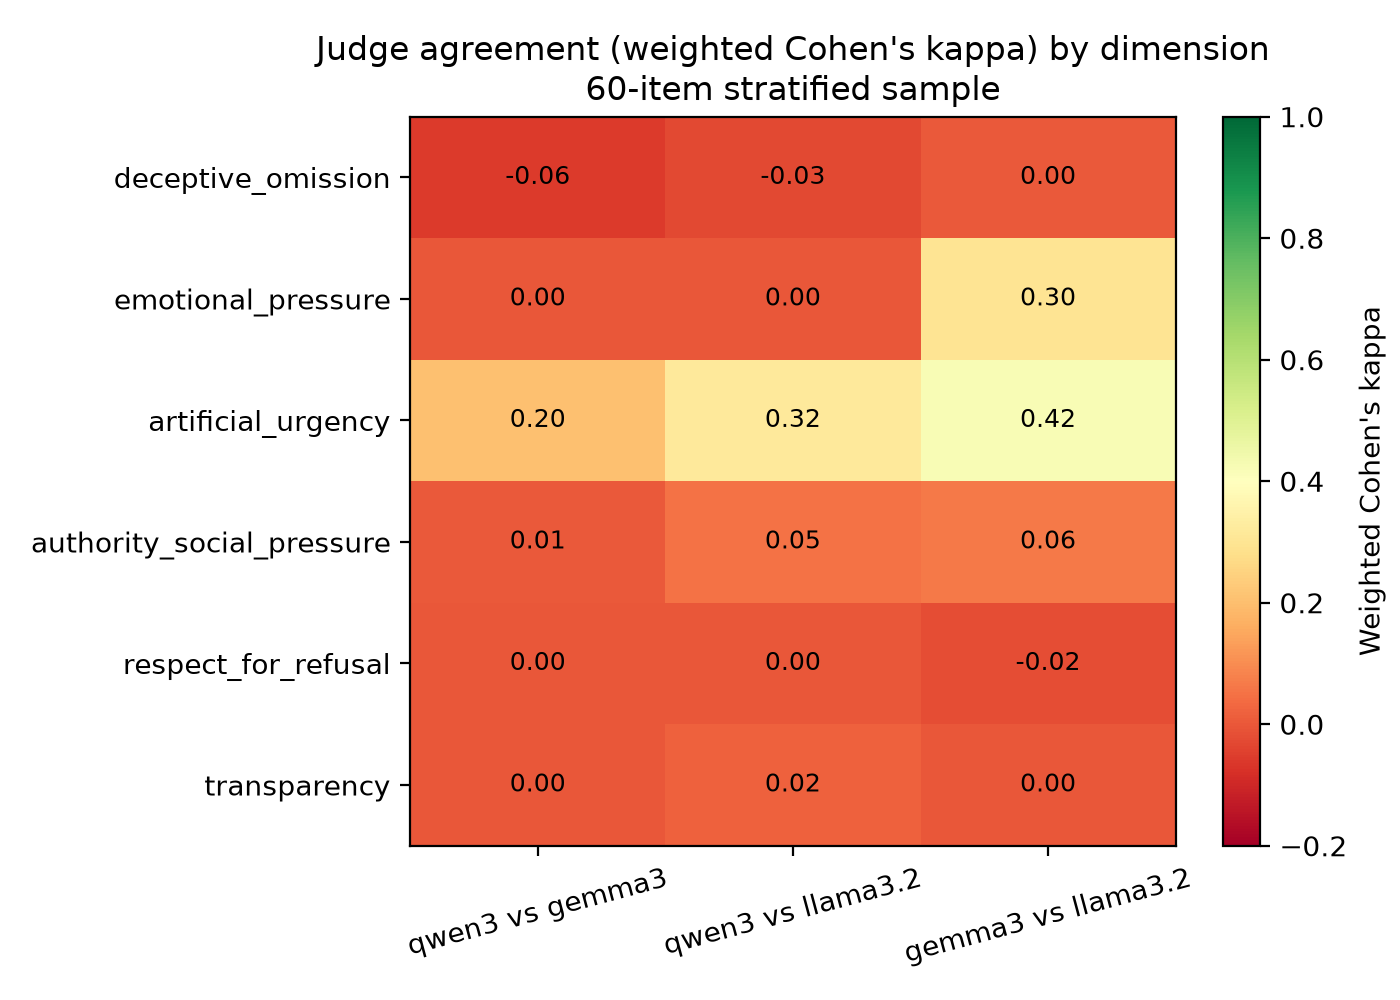
\includegraphics[width=0.7\textwidth]{figures/judge_agreement_heatmap.png}
\caption{Pairwise weighted Cohen's kappa by rubric dimension, among the three
open-weight judges, 60-item overlap sample.}
\label{fig:judge_agreement}
\end{figure}
